\section{Sistemas de Radiocomunicación por Satélite}
\label{sec:satelite}
	\subsubsection{Introducción e historia}
	\label{ssub:introSat}
		El objetivo delos sistemas de radiocomunicación por satelite es el establecimiento de enlaces entre estaciones, tanto fijas como móviles, mediante repetidores en la órbita terrestre. Este concepto se refleja ya en artículos desde 1929. Los repetidores pueden ser tanto activos como pasivos, es decir, pueden amplificar la señal o no.\\
		La carrera espacial empieza con la idea de utilizar el espacio para lo militar. En 1957 se lanzan los primeros Sputnik y a Laika. Mientras tanto en estados unidos crean la NASA, sin lanzar nada al espacio. A partir de 1958 se empiezan a lanzar satelites de comunicación de la NASA con el departamento de defensa yanki. El primero fue un repetidor pasivo. En 1963 se pone en orbita el primer satélite geoestacionario, el Syncom 2.\\
		En 1964 se crea INTELSAT, una organización de 11 paises para la creación de un sistema comercial mundial de telecomunicaciones vía satélite. En la actualidad es privado y lo componen 109 paises. El primer satélite fue el early bird (INTELSAT I).\\
		Los sistemas satélite son una alternativa a otros sistemas. Con 3 satélites geoestacionarios se puede cubrir toda la superficie terrestre. Los equipos de comunicación y control deben ser muy fiables, ya que, la reparación puede ser imposible, además de estar expuestos a gran cantidad de radiaciones. Tienen una vida util limitada por el fin del combustible usado para los motores, una vez sin combustible no se pueden reorientar y se envian a una órbita basura. Los sistemas satélite se suelen usar como complemento, por ejemplo, un cable submarino puede tener un sistema satélite de soporte.
	% subsubsection introSat (end)
	\subsubsection{Servicios de satélites}
	\label{ssub:serviciosSat}
		\begin{itemize}
			\item Servicio fijo: Enlaces entre dos puntos terrestres usando el satélite como repetidor.
			\item Servicio Móvil: Uno o más puntos fijos y móviles, como barcos, aviones y torres de control.
			\item Servicio de radiodifusión: Uno o más puntos fijos y terminales dispersos, como la televisión o la radio satélite.
			\item Servicio de radiodeterminación: Localización determinada por satélites, como los sistemas GPS o Galileo.
			\item Servicio de exploración de la tierra: desde mapas del tiempo (meteosat), creación de mapas hasta la exploración de recursos.
			\item Servicio de exploración del espacio: mediante el uso de telescopios o radiotelescopios como el Hubble.
			\item Servicio entre satélites: La comunicación entre satélites no tiene limitaciones físicas para el uso de ancho de banda, por ejemplo, a 60GHz el oxígeno absorbe la señal, en el espacio no.
		\end{itemize}
	% subsubsection serviciosSat (end)
	\subsubsection{Estructura del sistema de comunicación satélite}
	\label{ssub:estructSat}
		\begin{figure}[htp]
			\centering
			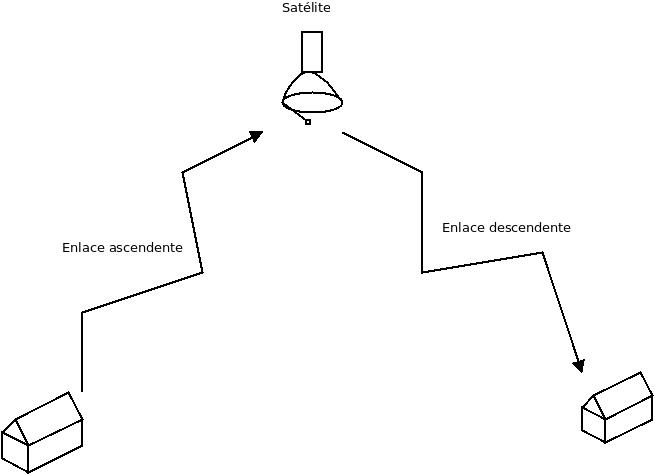
\includegraphics[width=0.7\textwidth]{Imagen/arquisatelite.jpg}
			\caption{Estructura de un sistema de comunicación satélite}
		\end{figure}
		\begin{itemize}
			\item Estación terrena de transmisión: Recibe la señal para posteriormente modularla a una radiofrecuencia (RF), amplificarla y después transmitirla. En transmisión se necesita mucha potencia y una gran directividad.
			\item Enlaces: tanto el enlace ascendente como el descendente se modelan como sistemas de transmisión en espacio libre con pérdidas ocasionadas por la frecuencia, distancia, atmosfera e incluso la lluvia.
			\item Satélite: Se trata de una estación repetidora, que amplifica, cambia de banda y retransmite las señales. Las partes involucradas en cada acción vienen descritas a continuación:
			\begin{itemize}
				\item Recepción: La antena, un filtro y un amplificador de bajo ruido.
				\item Transpondedor: Se trata de un conversor de frecuencia y amplificador encargado de llevar a cabo la retransmisión.
				\item Conmutación: piezas encargadas del encaminamiento y por tanto de la asignación de transpondedores.
				\item Transmisión: Amplificación, filtrado y antena de transmisión.
			\end{itemize}
			\item Estación terrena de recepción: Hace uso de un recptor superheterodino, receptor de ondas de radio que utiliza un proceso de mezcla de frecuencias o heterodinación para convertir la señal recibida en una a frecuencia intermedia. Esta señal sin la radioportadora de alta frecuencia es mucho más facil de manejar que la original.
			\item Segmento espacial: La suma de los retardos en los enlaces, en transmisión, en recepción y en el satélites terminan produciendo grandes retardos, 250ms en geoestacionarios. Este hecho hace necesario el uso de técnicas de cancelación de ecos.
		\end{itemize}
	% subsubsection estructSat (end)
% section satelite (end)